\documentclass{standalone}
\usepackage{tikz}
\usetikzlibrary{patterns, angles}
\usepackage{circuitikz}

\begin{document}
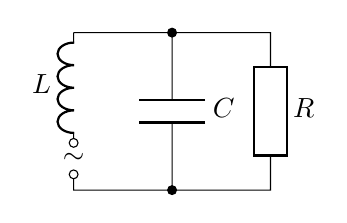
\begin{tikzpicture}[european]
	\draw (0,0) to [short,-*] (1.25,0) to [capacitor, l=$C$] (1.25, -2) to [short,*-] (0,-2) to [short,-o] (0,-1.8) (0,-1.4) to [american inductor,l =$L$, o-] (0,0)  (1.25,0) -- (2.5,0) to [R,l =$R$] (2.5, -2) -- (1.25,-2);
	\node at (0,-1.6) {$\sim$};
\end{tikzpicture}
\end{document}